\documentclass{article}


\usepackage{graphicx}
\usepackage{pgfplots}
\pgfplotsset{compat=1.9}
\pgfplotsset{major grid style={dashed,black}}
\pgfplotsset{minor grid style={solid,black}}
\usepackage{float}
%\usepackage{sidecap}
%\usepackage{csquotes} % ещё одна штука для цитат
\newtheorem{theorem}{Определение} % чтобы заработало окружение теорем

\usepackage[T2A]{fontenc}
\usepackage[utf8]{inputenc}
\usepackage[russian]{babel}
\usepackage{enumerate}
\usepackage{amsmath}

\newcommand{\rom}[1]
    {\MakeUppercase{\romannumeral #1}}

\usepackage{graphicx}
\title{Линейная Алгебра}
\author{Панов Петр Алексеевич}
\begin{document}
\maketitle
 
\tableofcontents

\section*{Структура курса}
\begin{itemize}
\item 3-4 модуль 1 курса
\begin{itemize}
\item КР - начало 4 модуля(0.3)
\item Экзамен - конец 4 модуля(0.5)
\item Текущая успеваемость - квизы, самостоятельные и т.д (0.2)
Можно компенсировать это выходом к доске, если проспал или плохо написал. Как работает разбалловка внутри этого пункта - одному Панову известно. Скорее всего, число СР+2=100%.
\end{itemize}

\item 1-2 модуль 2 курса
\begin{itemize}
\item КР - начало 2 модуля(0.3)
\item Экзамен - конец 2 модуля(0.5)
\item Текущая успеваемость - квизы, самостоятельные и т.д (0.2)
\end{itemize}
\item итоговая оценка - среднее арифметическое итогов 1 курса и 2 курса.
\end{itemize}

Блоков нет, все можно "переписать", если по уважительной причине прогулял - перед сессией.С неуважительными причинами - нельзя.

Материалы - в ЛМС.

\section*{Книги}
\begin{itemize}
\item Бурмистрова Лобанов - 1 часть
\item Хованская ирина Аскольдовна - курс на Курсере
\item
\end{itemize}

\section*{Введение}
Линейная алгебра изучает линейные пространства. Что это - пока не скажем, но к ним откосятся множество действительных и мнимых чисел, матриц и векторов.
\subsection*{Комплексные числа}
Это такие числа, которые содержат помимо действительной, еще и мнимую часть. Мнимая единица $i$ - число, такое, что $i^2=-1$. 
Соответственно, комплексное число имеет вид $a+bi$, $a$ - действительная часть, $b$ - мнимая.
Рассмотрим их свойства.

$$Z_1 = a_1 + b_1i, Z_2 = a_2 + b_2i$$
$$Z_1+Z_2 = (a_1+a_2) + (b_1+b_2)i$$
$$Z_1-Z_2 = (a_1-a_2) + (b_1-b_2)i$$
$$Z_1*Z_2 = (a_1a_2-b_1b_2) + (b_1a_2+a_1b_2)i$$
$$Z_1/Z_2 = \frac{a_1+b_1i}{a_2+b_2i} = \frac{(a_1+b_1i)(a_2-b_2i)}{a_2^2+b_2^2} = \frac{(a_1a_2+b_1b_2)}{a_2^2+b_2^2} + \frac{(b_1a_2-a_1b_2)i}{a_2^2+b_2^2}$$

Также комплексное число можно рассмотреть как точку на плоскости, аналогично тому, как действительное как точку на прямой. 
Точке (1023;65536) соответствует число $1023+65536i$, например. 

Модуль комплексного числа определен как длинна радиус-вектора, направленного из нуля в соответствующую точку и равен $\sqrt{a^2 + b^2}$.

Аргумент комплексного числа($Arg(Z) = \varphi$) - это угол между осью x и радиус-вектором этого числа. 
Ясно, что $\sin \varphi = \frac y{|Z|}$, $\cos \varphi = \frac x{|Z|}$, $\tan \varphi = \frac yx$

Еще один способ представления - через число  $e:

    $$z = r ( cos ⁡ \varphi + i sin ⁡ \varphi )$$ 
    
Еще один способ дает формула Эйлера:

    $$e ^{i \varphi}= cos ⁡ \varphi + i sin ⁡ \varphi$$
    
где $e$ — число Эйлера
Применяя эту формулу к тригонометрической форме, получим показательную форму комплексного числа:

    $$z = r e ^{i \varphi}$$
   
Следствия
\begin{itemize}
    \item Модуль выражения $e ^{i \varphi} $,  где \varphi вещественно, равен 1.
    \item $ \cos \varphi =\frac {e^{i\varphi }+e^{-i\varphi }}{2}$, 
    $ \sin \varphi =\frac {e^{i\varphi }-e^{-i\varphi }}{2i}$
\end{itemize}

Степени и корни:

$$ z^{n}=\left[r\left(\cos \varphi +i\sin \varphi \right)\right]^{n}=r^{n}\left(\cos n\varphi +i\sin n\varphi \right)$$,

$$z^{1/n}=\left[r\left(\cos \left(\varphi +2\pi k\right)+i\sin \left(\varphi +2\pi k\right)\right)\right]^{1/n}={\sqrt[{n}]{r}}\left(\cos {\frac {\varphi +2\pi k}{n}}+i\sin {\frac {\varphi +2\pi k}{n}}\right),\quad k=0,\;1,\;\ldots ,\;n-1.$$

Так что существуют корни любой степени, а их число равно степени.


\section*{Линейные преобразования}

Линейное преобразование - это преобразование, которое каждому элементу $R^n$ ставит элемент этого же $R^n$, причем $\varphi(a+b) = \varphi(a) + \varphi(b)$. 

На примере векторов из двух элементов:

$\varphi: (a,b) \to (3a, -5b)$ - линейное преобразование.
$\varphi: (a,b) \to (6a^3, b^7)$ - НЕ линейное преобразование

Каждое ЛП задается матрицей, и каждая матрица соответствует какому-то ЛП.

\subsection*{Матрицы}

$$ A=\begin{pmatrix}a_{11}&a_{12}&\cdots &a_{1n}\\a_{21}&a_{22}&\cdots &a_{2n}\\\vdots &\vdots &\ddots &\vdots \\a_{m1}&a_{m2}&\cdots &a_{mn}\end{pmatrix}}$$

Для матрицы определены следующие алгебраические операции:
\begin{itemize}
    \item сложение матриц, имеющих один и тот же размер;
    \item умножение матриц подходящего размера (матрицу, имеющую $n$ столбцов, можно умножить справа на матрицу, имеющую n {\displaystyle n} n строк);
    \item в том числе умножение на матрицу вектора (по обычному правилу матричного умножения; вектор является в этом смысле частным случаем матрицы);
    \item умножение матрицы на скаляр.
\end{itemize}

\subsubsetcion*{Сложение матриц}

Складывать можно только матрицы одинакового размера.

Сложение матриц  $A+B$ есть операция нахождения матрицы $C$, все элементы которой равны попарной сумме всех соответствующих элементов матриц $A$ и $B$, то есть каждый элемент матрицы $C$ равен

      $$ c_{ij} = a_{ij} + b_{ij}$$

Свойства сложения матриц:
\begin{itemize}
    \item коммутативность: $A+B = B+A$;
    \item ассоциативность: $(A+B)+C =A+(B+C)$;
    \item сложение с нулевой матрицей: $A + \Theta = A$;
    \item существование противоположной матрицы: $A + (-A) = \Theta$;
\end{itemize}

\subsubsection*{Умножение матрицы на число}

Умножение матрицы $A$ на число $\lambda \in R$ заключается в построении матрицы $\lambda A = ( \lambda a_{ij} )$.



Свойства умножения матриц на число:
\begin{itemize}
    \item умножение на единицу: $1A = A$;
    \item ассоциативность: $(\lambda\beta)A = \lambda(\beta A)$;
    \item дистрибутивность: $(\alpha+\beta)A = \alpha A + \beta A$;
    \item дистрибутивность: $\alpha(A+B) = \alpha A + \alpha B$;
\end{itemize}

\subsubsection*{Умножение матриц}
\begin{figure}
  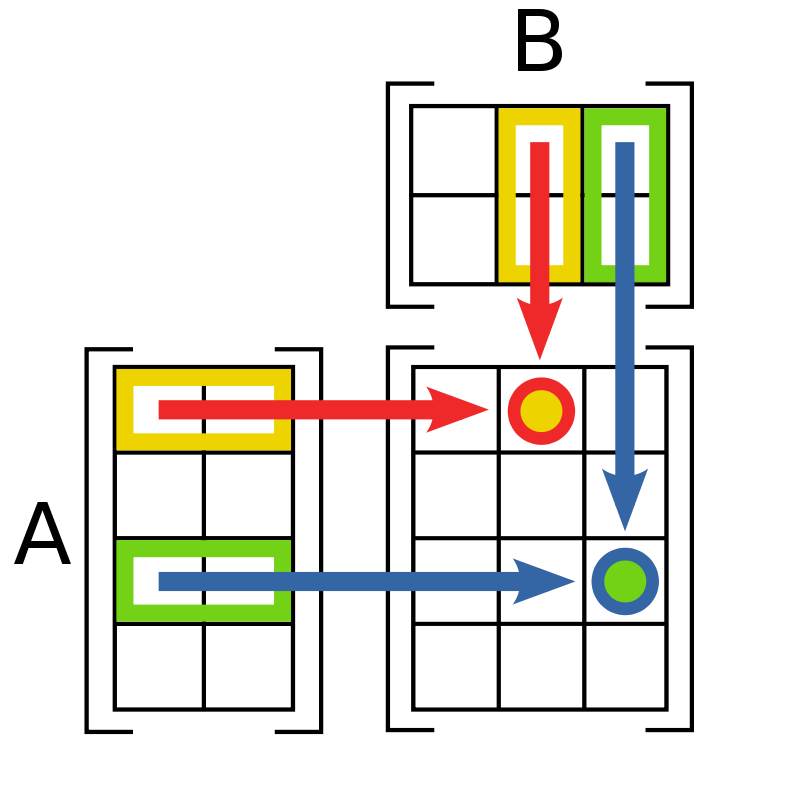
\includegraphics[width=0.6\linewidth]{matrix-multiplication.png}
  \caption{Умножение матриц}
\end{figure}
Умножение матриц (обозначение: $AB$, реже со знаком умножения $A\times B$ — есть операция вычисления матрицы $C$,
каждый элемент которой равен сумме произведений элементов в соответствующей строке первого множителя и столбце второго.

$$c_{ij}=\sum _{k=1}^{n}a_{ik}b_{kj}$$

Количество столбцов в матрице $A$ должно совпадать с количеством строк в матрице $B$, иными словами, 
матрица $A$ обязана быть согласованной с матрицей B {\displaystyle B} B. 
Если матрица $A$ имеет размерность $m\times n$, $B$ - $ n\times k$, 
то размерность их произведения $AB=C$ есть $m\times k$.

Свойства умножения матриц:

\begin{itemize}
    \item ассоциативность: $(AB)C = A(BC)$;
    \item некоммутативность (в общем случае): $AB \neq BA$;
    \item произведение коммутативно в случае умножения с единичной матрицей: $AI = IA$;
    \item дистрибутивность: $(A+B)C = AC + BC$, $A(B+C) = AB + AC$;
    \item ассоциативность и коммутативность относительно умножения на число: $(\lambda A)B = \lambda (AB) = A(\lambda B)$;
\end{itemize}

Для квадратных матриц существует единичная матрица E {\displaystyle E} E (аналог единицы для операции умножения чисел) такая,
что умножение любой матрицы на неё не влияет на результат, а именно $EA=AE=A$

У единичной матрицы единицы стоят только по главной диагонали, остальные элементы равны нулю

    $E=\begin{pmatrix}1&0&\cdots &0\\0&1&\cdots &0\\\vdots &\vdots &\ddots &\vdots \\0&0&\cdots &1\end{pmatrix}$


\end{docment}



